\section{Zielsetzung}
\label{sec:Zielsetzung}
Ziel dieses Experiments ist es, mittels Röntgenreflektivität die Strukturmerkmale
eines Polystyrolfilms auf einem Siliziumwafer zu analysieren. Die Analyse umfasst die 
Bestimmung der Dichte, Rauhigkeit und Schichtdicke des Films. Die gemessenen Daten liefern
Informationen über die Materialeigenschaften, die in der Mikroelektronik von großer Bedeutung sind.
Zudem soll ermittelt werden, wie effektiv Röntgenreflektivität zur Untersuchung von Grenzflächen auf festen 
und flüssigen Substraten eigesetzt werden kann.


\section{Theorie}
\label{sec:Theorie}
Röntgenstrahlung ist eine elektromagnetische Strahlung, die sich durch ihre hohe Energie und kurze 
Wellenlänge \(\lambda\) (0.01 bis 10 Nanometer) auszeichnet. Die Strahlung entsteht hauptsächlich durch 
Bremsstrahlung und durch charakteristische Röntgenstrahlung.

\subsection{Strahlungsarten}
Bremsstrahlung entsteht, wenn schnelle Elektronen in der Nähe von Atomkernen abgelenkt werden und dabei Energie
in Form von Photonen abgeben. Diese werden in eine Röntgenröhre beschleunigt und auf ein Metalltarget geschossen.
Beim Aufprall werden sie abgebremst und emittieren dabei Röntgenstrahlung. Diese Strahlung ist in dem Röntgenspektrum in
\ref{fig:Abbildung 1} mit dem kontinuierlichen Energiespektrum zu identifizieren.
Die charakteristische Röntgenstrahlung entsteht durch Übergänge von Elektronen in den Schalen von Atomen. Wenn Elektronen 
aus den inneren Schalen eines Atoms herrausgeschossen werden, füllen Elektronen aus höheren Schalen die frei gewordenen Plätze.
Während des Übergangs von Elektronen aus höheren Schalen in die freien Plätze der inneren Schalen wird die Differenz der
Energieniveaus der beiden Schalen in Form von Röntgenphotonen freigesetzt. Diese Energieemission entsteht, weil die Elektronen
beim Herabfallen auf ein niedrigeres Energieniveau überschüssige Energie abgeben, die als Röntgenstrahlung sichtbar wird. Die Strahlung 
zeigt ein diskretes Energiespektrum, das von den spezifischen Energieniveaus der Elektronen in den Atomen des Targets abhängt.


\begin{figure}
    \includegraphics[width=\textwidth]{bilder/Röntgenspektrum.jpg}
    \caption{Schematischer Abbildung des Röntgenspektrums}
    \label{fig:Abbildung 1}
\end{figure}
\cite{Röntgenspektrum}

\subsection{Verhalten an einer Grenzflächen}
Beim Einfall von Röntgenstrahlung auf eine glatte Grenzfläche wird diese durch den Brechungsindex des Mediums beeinflusst.
Der komplexe Brechungsindex wird beschrieben durch:
\begin{equation}
    n=1-\delta+i\beta
\end{equation}
Dabei ist der Parameter \(\delta\) eine sehr kleine Korrekturgröße im Bereich von $10^{-6}$
und gibt an, wie stark die Phasenverschiebung der Röntgenstrahlung beim Durchgang durch das Medium ist.
Diese Korrektur ist dimensionslos. Der imaginäre Teil \(i\beta\) beschreibt die Absorption der Strahlung im Material.
Hierbei steht \(\beta\) für den Absorptionskoeffizienten, je größer dieser ist, desto stärker wird die Strahlung absorbiert.

\begin{figure}
    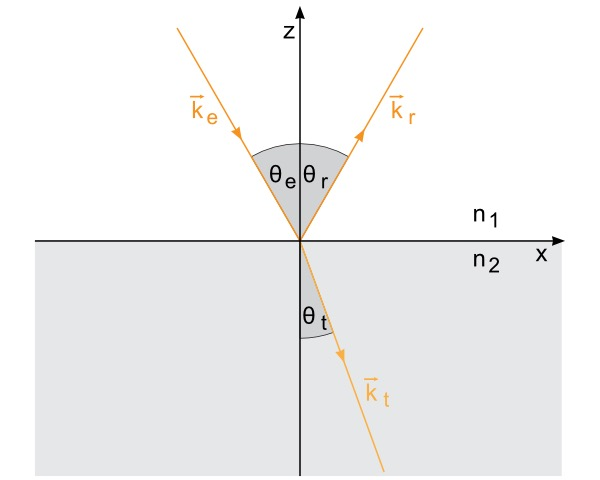
\includegraphics[width=\textwidth]{bilder/Reflexion.jpg}
    \caption{Skizze zum Verhalten elektromagnetischer Strahlung an einer Grenzschicht zwischen zwei Medien}
    \label{fig:Abbildung 2}
\end{figure}
\cite{Reflexion}

In \ref{fig:Abbildung 2} sind die Wellenvektoren der einfallenden $\vec{k}_e$, reflektierten $\vec{k}_r$ und der
transmittierten $\vec{k}_t$ Wellen sowie die entsprechenden Winkel zur Ebene $(\theta_e,\theta_r,\theta_t)$ dargestellt.
Das Snellius-Brechungsgesetzt besagt:
\begin{equation}
    n_1cos(\theta_e)=n_2cos(\theta_a)
\end{equation}
Wobei $\theta_a$ der Ausfallswinkel ist und $\theta_e=\theta_r$ gilt.    
Die Fresnelschen Formeln beschreiben die Amplitudenverhältnisse von senkrecht und parallel polarisiertem Licht
an einer Grenzfläche. Bei Röntgenstrahlung sind diese Verhältnisse für parallel und senkrecht polarisierten Anteil nahezu 
identisch. Das liegt daran, dass die die Brechungsindizes kaum Unterschiede aufweisen. 
Der Reflexionskoeffizient \(r\) gibt das Verhältnis der Amplitude der reflektierten Welle zur Amplitude der einfallenden Welle an. 
Er beschreibt, wie viel der einfallenden Welle an der Grenzfläche reflektiert wird. Der Betrag von \(r\) kann zwischen 0 und 1
liegen, wobei 0 bedeutet, dass keine Reflexion stattfindet und 1 bedeutet, dass die gesamte Welle reflektiert wird.
Der Transmissionskoeffizient \(t\) gibt das Verhältnis der Amplitude der transmittierten Welle zur Amplitude der einfallenden Welle an.
Er beschreibt, wie viel der einfallenden Welle die Grenzfläche durchdringt und in das zweite Medium gelangt. Auch hier kann der Betrag 
zwischen 0 und 1 liegen, wobei 0 bedeutet, dass keine Transmission stattfindet und 1 bedeutet, dass die gesamte Welle durchgelassen wird.
Diese Koeffizienten sind wie folgt definiert:
\begin{equation}
    r=\frac{n_1sin(\theta_i)-n_2sin(\theta_t)}{n_1sin(\theta_i)+n_2sin(\theta_t)}
\end{equation}
\begin{equation}
    t=\frac{2n_1sin(\theta_i)}{n_1sin(\theta_i)+n_2sin(\theta_t)} 
\end{equation}
Wenn das erste Medium Vakuum ist (n=1), tritt bei einem kritischen Winkel $\theta_c$ Totalreflexion auf, da der Brechungsindex von Materie für
Röntgenstrahlung immer kleiner als 1 ist. Dieser kritische Winkel kann näherungsweise durch folgende Gleichung bestimmt werden:
\begin{equation}
    \theta_c = \sqrt{2\delta} = \lambda \sqrt{\frac{r_e \rho}{\pi}}
\end{equation}    
dabei sind $\lambda$ die Wellenlänge der Röntgenstrahlung, \(r_e\) der klassische Elektronenradius und $\rho$ die Elektronendichte des Materials.
Für die Reflektivität \(R\), die das Verhältnis der Intensitäten der reflektierten und der einfallenden Welle beschreibt gilt:
\begin{equation}
    R=|r|^2
\end{equation}
Unter der Annahme dass $\theta_i>3\theta_c$ gilt:
\begin{equation}
    R=(\frac{\theta_c}{2\theta_i})^4
\end{equation} 
\cite{Röntgenstrahlung}.

\subsection{Göbelspiegel}
Der Göbelspiegel ist ein optisches Werkzeug, das in der  Röntgenreflektometrie verwendet wird um Röntgenstrahlen 
zu bündeln und zu fokussieren. Ein Göbelspiegel besteht aus einer Serie von ringförmigen Spiegeln, diese sind so angeordnet,
dass sie Röntgenstrahlen in einem flachen Winkel (ca 3°) reflektieren. Röntgenstrahlung haben kurze Wellenlängen und hohe Energien,
um Totalreflektion zu erreichen, muss der Einfallswinkel der Röntgenstrahlung flach sein, da der kritische Winkel für Totalreflektion
bei Röntgenstrahlung sehr klein ist. Dies liegt daran, dass der Brechungsindex für Röntgenstrahlen in den meisten Materialien sehr
nahe bei 1 liegt, was bedeutet, dass das Licht fast parallel zur Oberfläche reflektiert wird. Bei flachen Einfallswinkeln wird die Energie
der Röntgenstrahlen nahezu vollständig reflektiert, ohne signifikanten Verlust. Dies führt dazu, dass die Röntgenstrahlen effektiv gebündelt 
werden können, da die Reflexion an den Oberflächen der Ringspiegel mehrfach erfolgt, bevor die Strahlen fokussiert werden. Dies ermöglicht es,
mit einem eng gebündelten Strahl zu arbeiten, der dann zur präzisen Untersuchung von Proben verwendet werden kann.

\subsection{Röntgenstrahlung an Multischichtsystemen}

\begin{figure}
    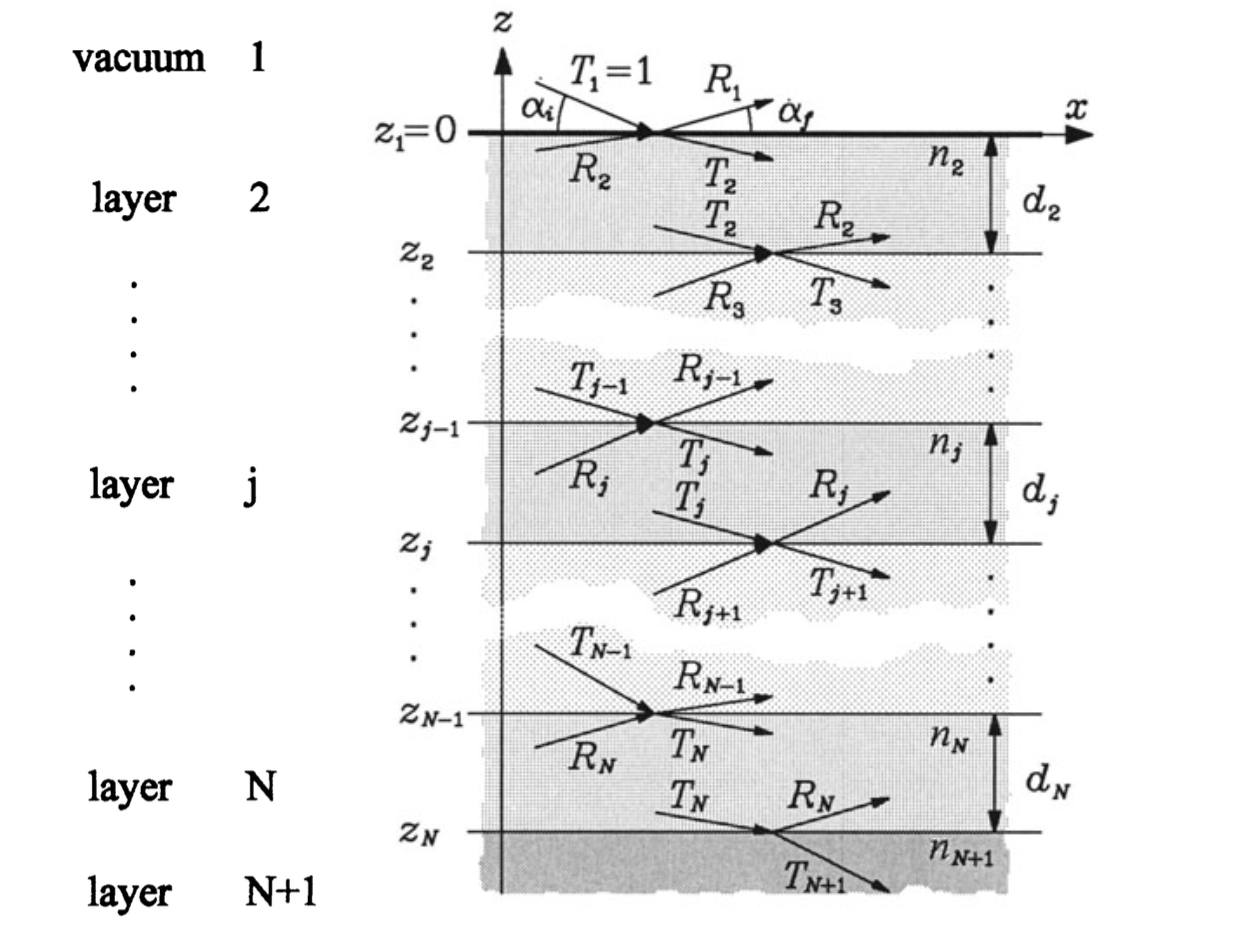
\includegraphics[width=\textwidth]{bilder/Multischichten.png}
    \caption{Skizze eines Systems aus N+1 Schichten mit N Grenzflächen. Es gilt $R_{N+1}=0$
    das heißt, dass es keine Reflexion vom Substrat gibt}
    \label{fig:Abbildung 3}
\end{figure}
\cite{Multischichten}

Bisher wurde nur das Verhalten von Röntgenstrahlung an einer einzelnen Grenzschicht untersucht, betrachtet man ein System 
welches aus mehreren Schichten besteht, werden die Strahlen an jeder Schicht teilweise reflektiert und transmittiert. Die
reflektierten Wellen interferieren miteinander und erzeugen ein Interferenzmuster. Die Phase der reflektierten Welle hängt von der Schichtdickeund dem 
Brechungsindex ab. Wenn die Phasendifferenz ein ganzzählig Vielfaches der Wellenlänge ist, tritt konstruktive Interferenz auf, was zu einem 
Maxima in der Reflexion führt. Die Positionen der Intensitätsmaxima können durch folgende Formel bestimmt werden:
\begin{equation}
    m\lambda=2ndsin(\theta)
\end{equation}
Dabei ist \(m\) eine ganze Zahl, \(d\) die Schichtdicke, \($\theta$\) der Einfallswinkel und \($\lambda$\) die Wellenlänge.  
Mithilfe der Kiessig-Oszillationen lässt sich die Dicke der Schicht über folgende Gleichung bestimmen:
\begin{equation}
    d=\frac{\lambda}{2\increment\alpha_i}
\end{equation}
Hierbei ist $\alpha_i$ der Abstand zweier Extrema welche das gleiche Vorzeichen haben.
Besteht das System aus mehr als zwei Schichten werden die Kiessig-Oszillationen überlagert, Mithilfe des Parratt-Algorithmus werden 
diese Überlagerungen quantisiert. Der Algorithmus basiert auf der rekursiven Berechnung der Reflexion an jeder Schicht und berücksichtigt 
die Reflexion an der Grenzfläche zwischen den Schichten sowie die Mehrfachreflexionen innerhalb eines Systems. Der Algorithmus beginnt 
mit dem Reflexionskoeffizienten zwischen dem Substrat und der ersten Schicht. Für jede weitere Schicht wird die Reflexion rekursiv berechnet, indem 
die Reflexion der vorherigen Schicht und der Transmissionskoeffizient der aktuellen Schicht verwendet werden. So erhält man den endgültigen Koeffizienten 
für das Multischichtsystem. Die Rekursionsformel lautet sieht wie folgt aus:
\begin{equation}
    X_j=\frac{R_j}{T_j}=exp(-2ik_{z,j}z_j)\frac{r_{j,j+1}+X_{j+1}exp(2ik_{z,j+1}z_j)}{1+r_{j,j+1}X_{j+1}exp(2ik_{z,j+1}z_j)}
\end{equation}
mit dem j-ten Reflexionskoeffizient aus den Fresnelschen Formeln
\begin{equation}
r_{j,j+1}=\frac{k_{z,j}-k_{z,j+1}}{k_{z,j}+k_{z,j+1}}
\end{equation}
Bei der Berechnung wird die unterste Schicht als unendlich Dick angenommen, so dass es keine Reflexion von weiter unten geben kann. 
\begin{equation}
R_{N+1}=X_{N+1}=0 
\end{equation}
Mit \(N\) als Gesamtanzahl der Schichten
\cite{Algorithmus}.

\subsubsection{Rauigkeit von Multischichtsystemen}

\begin{figure}
    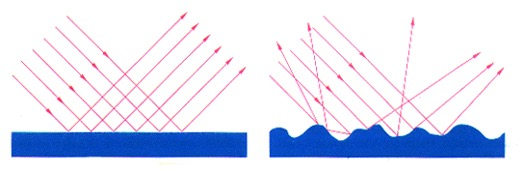
\includegraphics[width=\textwidth]{bilder/Rauigkeit.jpg}
    \caption{Reflexion von Strahlung an einer glatten Oberfläche im Vergleich zur Reflexion an einer rauen Oberfläche}
    \label{fig:Abbildung 4}
\end{figure}
\cite{Oberflächen}


In der Praxis sind Grenzschichten nicht perfekt glatt, sonder uneben. Diese Unebenheiten bezeichnet man als Rauigkeit.
Mathematisch kann die Rauigkeit als Varianz des Höhenfeldes einer Oberfläche beschrieben werden, sie gibt also an, wie Stark die einzelnen
Höhenwerte um den Durchschnittswert streuen. Die Varianz ist die quadrierte Standartabweichung $\sigma$ 
\begin{equation}
    \sigma^2_j=\int^{}(z-z_j)^2P_j(z)dz
\end{equation}
mit \(z_j\) der Position der j-ten Grenzschicht und \(P_j(z)\) der Wahrscheinlichkeit, dass die j-te
Grenzschicht im Intervall $[z_j+z,z_j+z+dz]$ liegt. Anschaulich ist diese Wahrscheinlichkeit eine Gauß-Glocke
mit der Breite $\sigma$. Die vorher definierten Fresnel-Koeffizienten sind nur für glatte Grenzflächen gültig, 
bei betrachtung von rauen Oberflächen müssen sie Mithilfe der Varianz $\sigma^2$ angepasst werden.
\begin{equation}
    \tilde{t}{_{j,j+1}}=t_{j,j+1}exp\Biggl(\frac{(k_{z,j}-k_{z,j+1})^{2}\sigma_j^2}{2}\Biggr)
\end{equation}

\begin{equation}
    \tilde{r}{_{j,j+1}}=r_{j,j+1}exp(-2k_{z,j}k_{z,j+1}\sigma_j^2)
\end{equation}

Mit diesen modifizierten Koeffizienten kann der Parratt-Algorithmus auch auf Raue Grenzfläöchen angewendet werden.
\subsection{Der Geometriefaktor}
Unter einem bestimmten Einfallswinkel unter dem Grenzwinkel $\alpha_c$ trifft nicht mehr der gesamte Röntgenstrahl
auf die Probe, sondern nurnoch ein Teil. Der Grenzwinkel ist abhängig von der Strahlbreite $d_0$ und der Länge der Probe \(D\)

\begin{equation}
    \alpha_c=arcsin\Bigl(\frac{d_0}{D}\Bigr)
\end{equation}

Um diesen Effekt zu berücksichtigen wird der Geometriefaktor \(G\) eingeführt

\begin{equation}
    G=
    \begin{cases}
        \frac{Dsin(\alpha_i)}{d_0}  &  \alpha_i < \alpha_c \\
        1                           & \alpha_i \ge \alpha_c \\

    \end{cases}
\end{equation}   


\cite{sample}
